\documentclass[10.5pt,a4paper]{article}
\usepackage[utf8]{vietnam}
\usepackage{amsmath,amssymb}
\usepackage{geometry}
\geometry{top=1.5cm,bottom=1.2cm,left=1.4cm,right=1.4cm,headheight=28pt,headsep=12pt,footskip=18pt}
\usepackage{tikz}
\usepackage{xcolor}
\usepackage{graphicx}
\usepackage{fancyhdr}
\usepackage{tabularx}
\usepackage{enumitem}
\usepackage{tcolorbox}
\usepackage{colortbl}
\usepackage[version=4]{mhchem}

\renewcommand{\baselinestretch}{1.12}
\setlength{\parskip}{2.5pt}
\setlength{\parindent}{0pt}

\definecolor{hfRed}{RGB}{211,47,47}
\definecolor{hfGreen}{RGB}{139,195,144}
\definecolor{myGreen}{RGB}{46,125,50}
\definecolor{myBlue}{RGB}{21,101,192}
\definecolor{myRed}{RGB}{198,40,40}

\tcbset{
  colback=blue!3!white,
  colframe=myBlue!60!black,
  boxrule=0.6pt,
  arc=2pt,
  left=4pt,
  right=4pt,
  top=3pt,
  bottom=3pt
}

\pagestyle{fancy}
\fancyhf{}
\fancyhead[L]{\small\itshape\color{hfRed} Tài liệu lưu hành nội bộ}
\fancyhead[R]{\small\color{hfRed} Thầy \textbf{TRẦN VĂN THẠNH} - 0777.470.803}
\renewcommand{\headrulewidth}{0.8pt}
\renewcommand{\headrule}{\hbox to\headwidth{\color{hfGreen}\leaders\hrule height \headrulewidth\hfill}}

\fancyfoot[L]{\small\itshape\color{hfRed} CS1: 6/15 Nguyễn Hoàng, P. Kim Long, TP Huế \quad|\quad CS2: 24 Đặng Thái Thân, TP Huế}
\fancyfoot[R]{\small\bfseries\color{hfRed} Trang \thepage}
\renewcommand{\footrulewidth}{0.8pt}
\renewcommand{\footrule}{\hbox to\headwidth{\color{hfGreen}\leaders\hrule height \footrulewidth\hfill}}

\newcommand{\loigiai}[1]{%
  \vspace{1pt}
  \begin{tcolorbox}
  {\color{myBlue}\bfseries Lời giải chi tiết:}\par\vspace{1pt}
  {\small #1}
  \end{tcolorbox}
  \vspace{2pt}
}

\begin{document}

% --- TITLE BLOCK ---
\begin{tabularx}{\textwidth}{@{}l X r@{}}
\textbf{\small SỞ GD \& ĐT GIA LAI} & & \textbf{\small ĐỀ KIỂM TRA GIỮA KỲ I, NĂM HỌC 2024 - 2025} \\
\textbf{\normalsize TRƯỜNG THPT SỐ 2 QUANG TRUNG} & & \textbf{\normalsize MÔN: HOÁ HỌC; KHỐI 11} \\
\textbf{\small ĐỀ CHÍNH THỨC} & & \textbf{\small Thời gian làm bài: 45 phút} \textit{(không kể thời gian phát đề)} \\
\textit{\small (Đề thi có 04 trang)} & & \textbf{\normalsize MÃ ĐỀ: 1202}
\end{tabularx}

\begin{center}
{\color{myRed}\bfseries (BẢN GIÁO VIÊN -- CÓ ĐÁP ÁN \& LỜI GIẢI CHI TIẾT)}\par\vspace{2pt}
\textit{Họ, tên thí sinh:} \dotfill \quad \textit{Lớp:} \dots\dots\dots \quad \textit{Số báo danh:} \dotfill
\end{center}

\vspace{-2pt}
\noindent\textit{\small (Cho biết nguyên tử khối: C = 12; H = 1; O = 16; S = 32; Fe = 56).}
\vspace{-2pt}
\noindent{\color{gray!50}\hrule height 0.8pt}
\vspace{6pt}

% =========================================================================
% PHẦN I
% =========================================================================
{\color{myGreen}\large\bfseries PHẦN I. CÂU TRẮC NGHIỆM NHIỀU PHƯƠNG ÁN LỰA CHỌN (4,0 điểm)}

\textit{Học sinh trả lời từ câu 1 đến câu 16. Mỗi câu hỏi học sinh chỉ chọn một phương án đúng.}

\vspace{2pt}
\textbf{Câu 1:} Cho phản ứng hoá học: \ce{CO2(g) + H2(g) <=> CO(g) + H2O(g)}. Biểu thức hằng số cân bằng ($K_C$) của phản ứng trên là
\begin{enumerate}[label=\textbf{\Alph*.}, itemsep=1pt, topsep=1pt, leftmargin=1.5cm]
    \item $K_C = \dfrac{[\ce{H2}][\ce{CO}]}{[\ce{CO2}][\ce{H2O}]}$ \hfill \item \textbf{\color{myRed}$K_C = \dfrac{[\ce{H2O}][\ce{CO}]}{[\ce{CO2}][\ce{H2}]}$} \hfill \item $K_C = \dfrac{[\ce{CO2}][\ce{CO}]}{[\ce{H2O}][\ce{H2}]}$ \hfill \item $K_C = \dfrac{[\ce{CO2}][\ce{H2}]}{[\ce{CO}][\ce{H2O}]}$
\end{enumerate}
\loigiai{Theo định luật tác dụng khối lượng: $K_C = \dfrac{[\ce{CO}][\ce{H2O}]}{[\ce{CO2}][\ce{H2}]}$.\\ \textbf{$\implies$ Chọn B.}}

\textbf{Câu 2:} Phản ứng thuận nghịch là phản ứng:
\begin{enumerate}[label=\textbf{\Alph*.}, itemsep=1pt, topsep=1pt, leftmargin=1.5cm]
    \item \textbf{\color{myRed}xảy ra theo hai chiều ngược nhau trong cùng điều kiện.}
    \item xảy ra theo một chiều duy nhất trong điều kiện xác định.
    \item có phương trình hoá học được biểu diễn bằng mũi tên một chiều.
    \item xảy ra theo hai chiều giống nhau trong cùng điều kiện xác định.
\end{enumerate}
\loigiai{Theo định nghĩa SGK Hóa học 11, phản ứng thuận nghịch là phản ứng xảy ra theo hai chiều ngược nhau trong cùng điều kiện.\\ \textbf{$\implies$ Chọn A.}}

\textbf{Câu 3:} Sulfur là nguyên tố phổ biến thứ 17 trên vỏ Trái Đất, tồn tại ở bốn dạng đồng vị bền. Đồng vị chiếm \% về khối lượng cao nhất là:
\begin{enumerate}[label=\textbf{\Alph*.}, itemsep=1pt, topsep=1pt, leftmargin=1.5cm]
    \item \textbf{\color{myRed}$^{32}_{16}\ce{S}$.} \hfill \item $^{34}_{16}\ce{S}$. \hfill \item $^{36}_{16}\ce{S}$. \hfill \item $^{33}_{16}\ce{S}$.
\end{enumerate}
\loigiai{Trong tự nhiên, $^{32}_{16}\ce{S}$ chiếm hàm lượng cao nhất (khoảng $94,98\%$).\\ \textbf{$\implies$ Chọn A.}}

\textbf{Câu 4:} Biểu thức tính pH đúng là
\begin{enumerate}[label=\textbf{\Alph*.}, itemsep=1pt, topsep=1pt, leftmargin=1.5cm]
    \item $\text{pH} = +10 \lg[\ce{H+}]$. \hfill \item $\text{pH} = -\lg[\ce{OH-}]$. \hfill \item $\text{pH} = \lg[\ce{H+}]$. \hfill \item \textbf{\color{myRed}$\text{pH} = -\lg[\ce{H+}]$.}
\end{enumerate}
\loigiai{Theo định nghĩa: $\text{pH} = -\lg[\ce{H+}]$.\\ \textbf{$\implies$ Chọn D.}}

\textbf{Câu 5:} Cân bằng hoá học nào sau đây bị chuyển dịch khi thay đổi áp suất?
\begin{enumerate}[label=\textbf{\Alph*.}, itemsep=1pt, topsep=1pt, leftmargin=1.5cm]
    \item \ce{3Fe(s) + 4H2O(g) <=> Fe3O4(s) + 4H2(g)}
    \item \textbf{\color{myRed}\ce{C(s) + H2O(g) <=> CO(g) + H2(g)}}
    \item \ce{C(s) + O2(g) <=> CO2(g)}
    \item \ce{H2(g) + I2(g) <=> 2HI(g)}
\end{enumerate}
\loigiai{Phản B có $\Delta n_{\text{khí}} = (1 + 1) - 1 = +1 \neq 0$ nên cân bằng bị chuyển dịch khi áp suất thay đổi.\\ \textbf{$\implies$ Chọn B.}}

\textbf{Câu 6:} Trong tự nhiên, nguyên tố sulfur
\begin{enumerate}[label=\textbf{\Alph*.}, itemsep=1pt, topsep=1pt, leftmargin=1.5cm]
    \item chỉ tồn tại ở dạng hợp chất. \hfill \item \textbf{\color{myRed}tồn tại ở cả dạng đơn chất và dạng hợp chất.}
    \item chỉ tồn tại ở dạng đơn chất. \hfill \item chỉ sinh ra khi núi lửa hoạt động ở dạng khí \ce{SO2}.
\end{enumerate}
\loigiai{Sulfur trong tự nhiên tồn tại ở dạng đơn chất (các mỏ lưu huỳnh tự do) và dạng hợp chất (quặng sulfide, sulfate, protein sinh học).\\ \textbf{$\implies$ Chọn B.}}

\textbf{Câu 7:} Ứng dụng không phải của ammonia là
\begin{enumerate}[label=\textbf{\Alph*.}, itemsep=1pt, topsep=1pt, leftmargin=1.5cm]
    \item \textbf{\color{myRed}Sản xuất sulfuric acid.} \hfill \item Sử dụng làm dung môi.
    \item Sản xuất nitric acid. \hfill \item Sản xuất phân bón như: đạm, ammophos.
\end{enumerate}
\loigiai{Sulfuric acid (\ce{H2SO4}) được sản xuất từ sulfur hoặc pyrite, không dùng ammonia.\\ \textbf{$\implies$ Chọn A.}}

\textbf{Câu 8:} Sulfur dioxide (\ce{SO2}) là một trong những chất gây ô nhiễm khí quyển phổ biến. Biện pháp nào sau đây không thể giảm phát thải \ce{SO2}?
\begin{enumerate}[label=\textbf{\Alph*.}, itemsep=1pt, topsep=1pt, leftmargin=1.5cm]
    \item Có biện pháp tái chế các sản phẩm phụ có chứa sulfur.
    \item Phát triển các nguồn năng lượng sạch, thân thiện với môi trường.
    \item \textbf{\color{myRed}Sử dụng các nguồn nhiên liệu như than đá, dầu mỏ.}
    \item Xây dựng hệ thống xử lí khí thải tại các nhà máy, khu công nghiệp.
\end{enumerate}
\loigiai{Than đá và dầu mỏ chứa tạp chất sulfur, khi đốt cháy sẽ thải thêm nhiều \ce{SO2}.\\ \textbf{$\implies$ Chọn C.}}

\begin{minipage}{0.68\textwidth}
\textbf{Câu 9:} Học sinh X thực hiện thí nghiệm chuẩn độ dung dịch \ce{NaOH} chưa biết chính xác nồng độ bằng dung dịch chuẩn \ce{HCl} 0,1 M với chỉ thị phenolphthalein. Lấy 10,00 mL dung dịch \ce{HCl} 0,1 M cho vào bình tam giác cùng với 1--2 giọt phenolphthalein.\\
Kết quả ghi lại thể tích \ce{NaOH} qua 3 lần chuẩn độ như sau:
\begin{center}
\begin{tabular}{|l|c|c|c|}
\hline
\textbf{Thí nghiệm} & 1 & 2 & 3 \\
\hline
\textbf{Thể tích NaOH (mL)} & 19,85 & 19,95 & 20,20 \\
\hline
\end{tabular}
\end{center}
Nồng độ (mol/L) của dung dịch \ce{NaOH} trong thí nghiệm trên là:
\end{minipage}
\hfill
\begin{minipage}{0.30\textwidth}
\centering
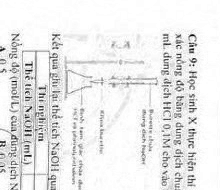
\includegraphics[width=0.85\textwidth]{images_de_1202/chuan_do_clean.png}
\end{minipage}

\begin{enumerate}[label=\textbf{\Alph*.}, itemsep=1pt, topsep=1pt, leftmargin=1.5cm]
    \item 0,5. \hfill \item \textbf{\color{myRed}0,05.} \hfill \item 0,1. \hfill \item 0,06.
\end{enumerate}
\loigiai{$\overline{V}_{\ce{NaOH}} = \dfrac{19,85 + 19,95 + 20,20}{3} = 20,00\text{ mL} = 0,020\text{ L}$.\\
Tại điểm tương đương: $n_{\ce{NaOH}} = n_{\ce{HCl}} = 0,1 \times 0,010 = 10^{-3}\text{ mol}$.\\
$C_{\ce{NaOH}} = \dfrac{10^{-3}}{0,020} = 0,05\text{ M}$.\\ \textbf{$\implies$ Chọn B.}}

\textbf{Câu 10:} Thực hiện thí nghiệm: Sulfur tác dụng với oxygen\\
\textit{Chuẩn bị:} bột sulfur, bình khí oxygen, muôi sắt, đèn cồn, nút cao su.\\
\textit{Tiến hành:}
\begin{itemize}[itemsep=0pt, topsep=1pt, leftmargin=0.8cm]
    \item Lấy một ít bột sulfur vào muôi sắt (đã cắm xuyên qua nút cao su).
    \item Hơ nóng muôi sắt trên ngọn lửa đèn cồn đến khi sulfur nóng chảy và cháy một phần trong không khí.
    \item Đưa nhanh muôi sắt vào bình khí oxygen.
\end{itemize}
Kết luận nào sau là không phù hợp?
\begin{enumerate}[label=\textbf{\Alph*.}, itemsep=1pt, topsep=1pt, leftmargin=1.5cm]
    \item Nếu đốt cháy hoàn toàn 6,4 gam sulfur trong oxygen dư thì thể tích \ce{SO2} (ở đkc) thu được là 4,958 L.
    \item Sulfur tác dụng với oxygen tạo thành hợp chất oxide acid (acidic oxide).
    \item \textbf{\color{myRed}Phản ứng chứng minh sulfur bị khử bởi oxygen.}
    \item Sulfur cháy mạnh hơn khi đưa vào bình khí oxygen.
\end{enumerate}
\loigiai{$\overset{0}{\text{S}} + \text{O}_2 \xrightarrow{t^\circ} \overset{+4}{\text{S}}\text{O}_2$. Sulfur tăng số oxi hóa từ 0 lên +4 nên là chất khử, tức sulfur bị oxi hóa bởi oxygen (chứ không phải bị khử).\\ \textbf{$\implies$ Chọn C.}}

\textbf{Câu 11:} Nitrogen monoxide được tạo thành khi mưa dông kèm theo sấm sét do phản ứng giữa nitrogen và oxygen trong không khí được gọi là:
\begin{enumerate}[label=\textbf{\Alph*.}, itemsep=1pt, topsep=1pt, leftmargin=1.5cm]
    \item \ce{NO_x} nhiên liệu. \hfill \item \ce{NO_x} tự nhiên. \hfill \item \textbf{\color{myRed}\ce{NO_x} nhiệt.} \hfill \item \ce{NO_x} tức thời.
\end{enumerate}
\loigiai{\ce{NO_x} hình thành do phản ứng trực tiếp giữa \ce{N2} và \ce{O2} ở nhiệt độ cực cao (hoặc sấm sét) được gọi là thermal \ce{NO_x} (\ce{NO_x} nhiệt).\\ \textbf{$\implies$ Chọn C.}}

\textbf{Câu 12:} Sự điện li là quá trình:
\begin{enumerate}[label=\textbf{\Alph*.}, itemsep=1pt, topsep=1pt, leftmargin=1.5cm]
    \item phân li các chất trong nước thành các chất đơn giản.
    \item \textbf{\color{myRed}phân li các chất trong nước tạo thành ion.}
    \item phân li các chất trong nước thành phần tử nhỏ hơn.
    \item hòa tan các chất trong nước.
\end{enumerate}
\loigiai{Sự điện li là quá trình phân li các chất trong nước tạo thành cation và anion.\\ \textbf{$\implies$ Chọn B.}}

\textbf{Câu 13:} Đo pH của một cốc nước chanh được giá trị pH bằng 2,4. Nhận định nào sau đây là đúng?
\begin{enumerate}[label=\textbf{\Alph*.}, itemsep=1pt, topsep=1pt, leftmargin=1.5cm]
    \item Nước chanh có môi trường base. \hfill \item Nước chanh làm phenolphthalein hóa màu hồng.
    \item Nước chanh làm giấy quỳ tím hóa xanh. \hfill \item \textbf{\color{myRed}Nước chanh làm giấy quỳ tím hóa đỏ.}
\end{enumerate}
\loigiai{$\text{pH} = 2,4 < 7$ nên môi trường acid, làm quỳ tím hóa đỏ.\\ \textbf{$\implies$ Chọn D.}}

\textbf{Câu 14:} Cặp kim loại nào sau đều không phản ứng được với nitric acid?
\begin{enumerate}[label=\textbf{\Alph*.}, itemsep=1pt, topsep=1pt, leftmargin=1.5cm]
    \item Fe, Mg. \hfill \item Ag, Al. \hfill \item Cu, Zn. \hfill \item \textbf{\color{myRed}Au, Pt.}
\end{enumerate}
\loigiai{Vàng (Au) và bạch kim (Pt) không phản ứng với dung dịch \ce{HNO3} ở bất kì nồng độ nào.\\ \textbf{$\implies$ Chọn D.}}

\begin{minipage}{0.75\textwidth}
\textbf{Câu 15:} Dựa vào công thức cấu tạo của nitric acid bên cạnh:\\
Cho biết phát biểu nào sau đây không đúng?
\begin{enumerate}[label=\textbf{\Alph*.}, itemsep=1pt, topsep=1pt, leftmargin=1.0cm]
    \item \textbf{\color{myRed}Liên kết O--H phân cực mạnh về phía nguyên tử hydrogen.}
    \item Liên kết \ce{N -> O} là liên kết cho nhận.
    \item Công thức phân tử nitric acid là \ce{HNO3}.
    \item Nguyên tử N có số oxi hóa +5, là số oxi hóa cao nhất của nitrogen.
\end{enumerate}
\end{minipage}
\hfill
\begin{minipage}{0.22\textwidth}
\centering
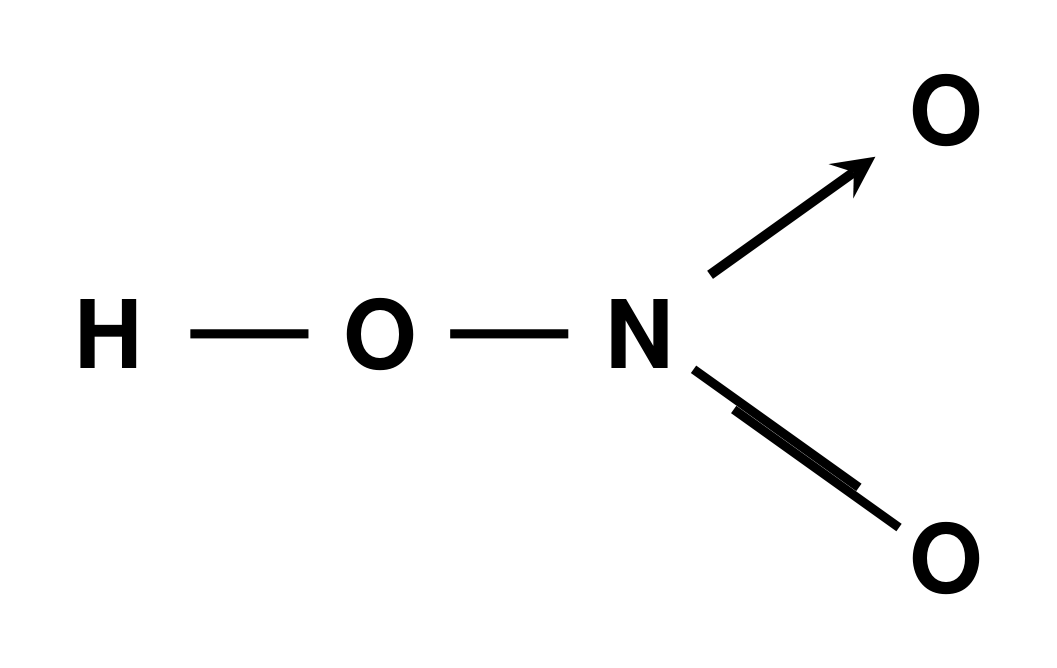
\includegraphics[width=0.95\textwidth]{images_de_1202/hno3_hd.png}
\end{minipage}
\loigiai{Độ âm điện của Oxygen lớn hơn Hydrogen nên cặp e dùng chung lệch mạnh về phía oxygen (chứ không phải hydrogen). Phát biểu A sai.\\ \textbf{$\implies$ Chọn A.}}

\textbf{Câu 16:} Ở trong tự nhiên, nguyên tố nitrogen tồn tại ở dạng:
\begin{enumerate}[label=\textbf{\Alph*.}, itemsep=1pt, topsep=1pt, leftmargin=1.5cm]
    \item chỉ ở dạng đơn chất. \hfill \item chỉ ở dạng hợp chất. \hfill \item chỉ ở dạng ion nitrate. \hfill \item \textbf{\color{myRed}cả đơn chất và hợp chất.}
\end{enumerate}
\loigiai{Nitrogen tồn tại cả ở dạng đơn chất (\ce{N2} trong không khí) và dạng hợp chất (khoáng diêm tiêu, protein...).\\ \textbf{$\implies$ Chọn D.}}

\vspace{6pt}
% =========================================================================
% PHẦN II
% =========================================================================
{\color{myGreen}\large\bfseries PHẦN II. CÂU TRẮC NGHIỆM ĐÚNG SAI (2,0 điểm)}

\textit{Học sinh trả lời từ câu 1 đến câu 2. Trong mỗi ý a), b), c), d) ở mỗi câu, học sinh chọn đúng hoặc sai.}

\vspace{2pt}
\textbf{Câu 1:} Dung dịch X chứa \ce{H2SO4} 0,05 M ở 25$^\circ$C. Xét từng phát biểu sau đây là đúng hay sai?
\begin{enumerate}[label=\textbf{\alph*)}, itemsep=1.5pt, topsep=1pt, leftmargin=0.8cm]
    \item \ce{H2SO4} là chất điện li mạnh. \hfill {\color{myRed}\textbf{$\implies$ (Đúng)}}
    \item Theo thuyết Brønsted -- Lowry, \ce{H2SO4} đóng vai trò acid vì có khả năng nhận proton (\ce{H+}). \hfill {\color{myRed}\textbf{$\implies$ (Sai)}}
    \item Dung dịch X làm phenolphthalein chuyển màu hồng. \hfill {\color{myRed}\textbf{$\implies$ (Sai)}}
    \item Trộn 300 mL dung dịch chứa \ce{NaOH} 0,15 M và \ce{Ba(OH)2} 0,05 M với 200 mL dung dịch X trên thu được 500 mL dung dịch có pH = 13 \textit{(Kết quả đã làm tròn số đến phần nguyên)}. \hfill {\color{myRed}\textbf{$\implies$ (Đúng)}}
\end{enumerate}
\loigiai{
a) \textbf{Đúng:} \ce{H2SO4} phân li hoàn toàn nấc 1 và gần như hoàn toàn nấc 2, là chất điện li mạnh.\\
b) \textbf{Sai:} Theo Brønsted -- Lowry, acid là chất \textbf{cho proton} (\ce{H+}), chứ không phải nhận proton.\\
c) \textbf{Sai:} Môi trường acid phenolphthalein không đổi màu (không màu).\\
d) \textbf{Đúng:} $\sum n_{\ce{OH-}} = 0,3 \times 0,15 + 2 \times (0,3 \times 0,05) = 0,075\text{ mol}$.\\
$n_{\ce{H+}} = 2 \times (0,2 \times 0,05) = 0,02\text{ mol}$.\\
$n_{\ce{OH- dư}} = 0,075 - 0,02 = 0,055\text{ mol} \implies [\ce{OH-}] = \dfrac{0,055}{0,5} = 0,11\text{ M}$.\\
$\text{pOH} = -\lg(0,11) \approx 0,96 \implies \text{pH} = 14 - 0,96 = 13,04 \approx 13$.
}

\textbf{Câu 2:} Hình 5.1 dưới đây mô tả công thức Lewis và dạng hình học của phân tử ammonia.
\begin{center}
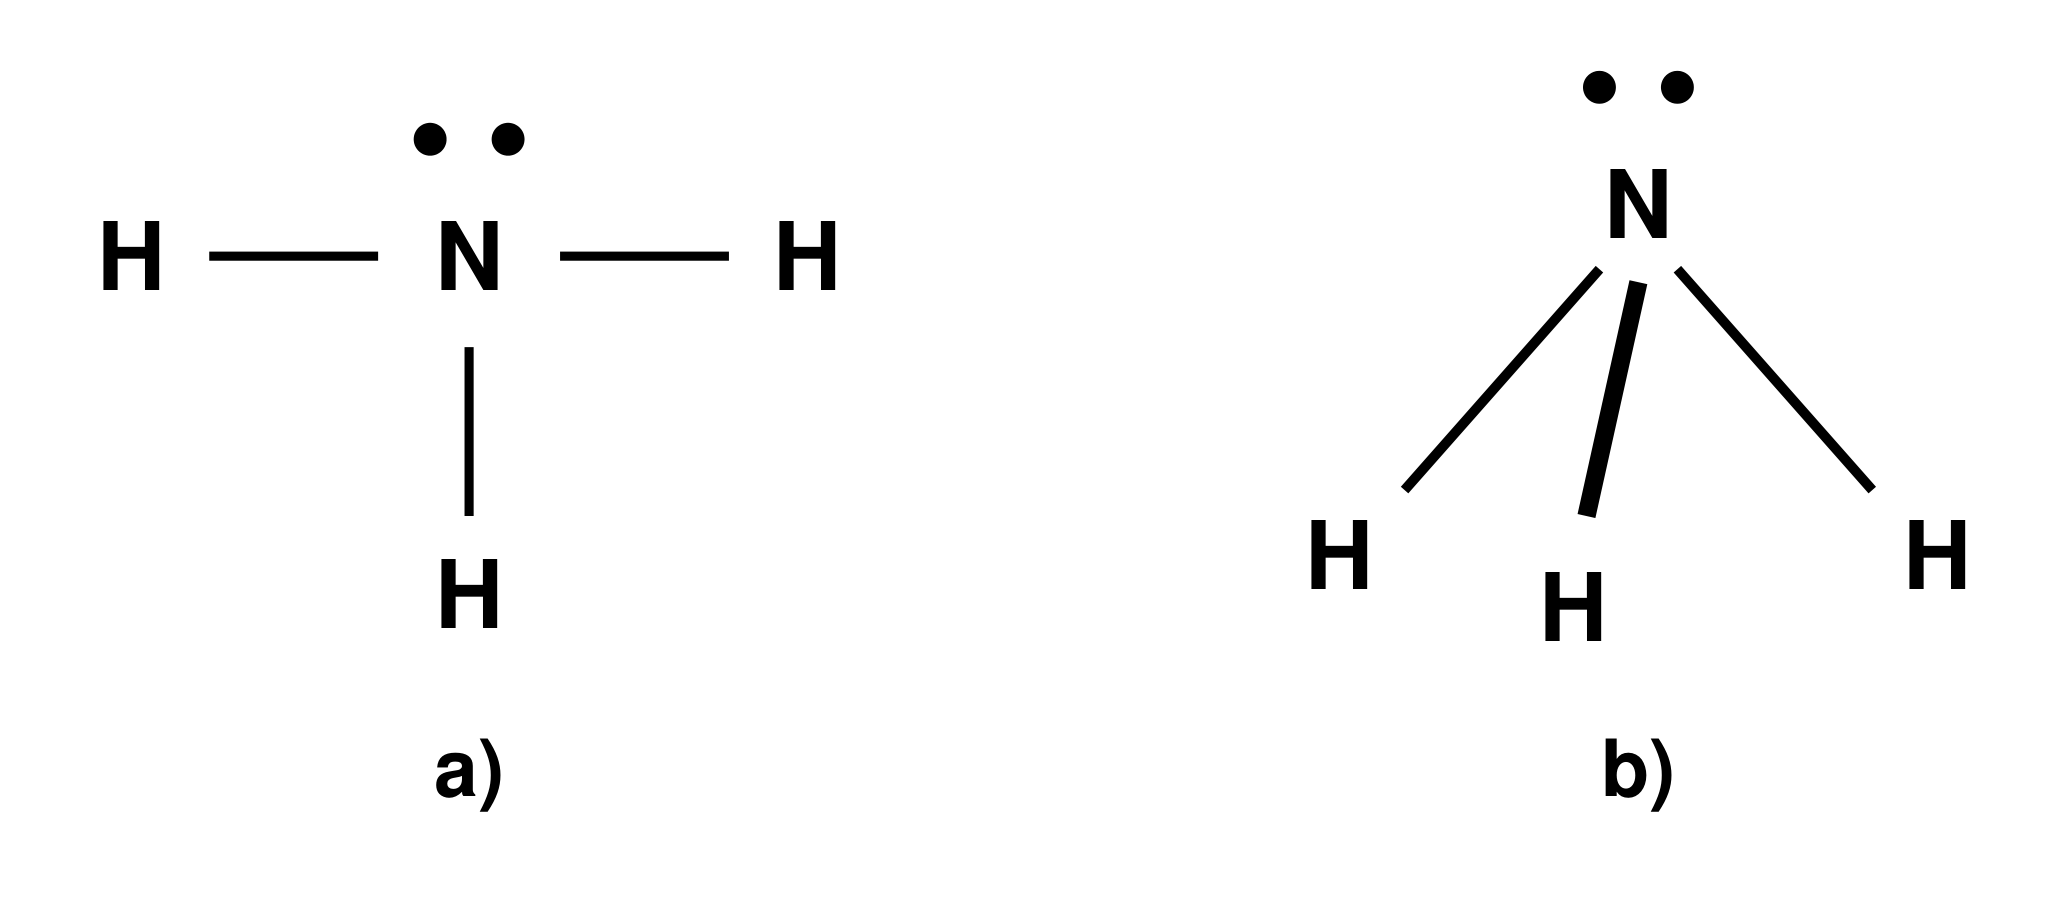
\includegraphics[width=0.45\textwidth]{images_de_1202/nh3_hd.png}\\
\textit{\small Hình 5.1. Công thức Lewis (a) và dạng hình học (b) của phân tử ammonia}
\end{center}
\begin{enumerate}[label=\textbf{\alph*)}, itemsep=1.5pt, topsep=1pt, leftmargin=0.8cm]
    \item Trong công nghiệp, ammonia thường được sử dụng đối với vai trò tác nhân làm lạnh (chất sinh hàn). \hfill {\color{myRed}\textbf{$\implies$ (Đúng)}}
    \item Trong công nghiệp, phản ứng giữa \ce{NH3} với acid được dùng để sản xuất phân bón. \hfill {\color{myRed}\textbf{$\implies$ (Đúng)}}
    \item \ce{NH3} tan nhiều trong nước chủ yếu do phân tử \ce{NH3} phân cực, có khả năng tạo liên kết hydrogen mạnh với nước. \hfill {\color{myRed}\textbf{$\implies$ (Đúng)}}
    \item Phương trình hoá học của phản ứng tổng hợp ammonia từ nitrogen và hydrogen bằng quá trình Haber như sau:\\
    \ce{N2(g) + 3H2(g) <=> 2NH3(g)} \quad $\Delta_r H^\circ_{298} = -91,8\text{ kJ}$.\\
    Nếu giảm áp suất của hệ thì cân bằng sẽ chuyển dịch theo chiều thuận, làm tăng hiệu suất tổng hợp \ce{NH3}. \hfill {\color{myRed}\textbf{$\implies$ (Sai)}}
\end{enumerate}
\loigiai{
a) \textbf{Đúng:} \ce{NH3} dễ hóa lỏng, nhiệt hóa hơi lớn nên dùng làm chất sinh hàn.\\
b) \textbf{Đúng:} Phản ứng tạo các loại muối amoni dùng làm phân bón.\\
c) \textbf{Đúng:} Tạo liên kết hydrogen mạnh với nước nên 1 lít nước hòa tan khoảng 700 lít \ce{NH3}.\\
d) \textbf{Sai:} Giảm áp suất cân bằng chuyển dịch theo chiều tăng số mol khí (chiều nghịch: từ 2 mol lên 4 mol), làm giảm hiệu suất tổng hợp.
}

\vspace{6pt}
% =========================================================================
% PHẦN III
% =========================================================================
{\color{myGreen}\large\bfseries PHẦN III. CÂU TRẮC NGHIỆM TRẢ LỜI NGẮN (2,0 điểm)}

\textit{Học sinh trả lời từ câu 1 đến câu 4.}

\vspace{2pt}
\textbf{Câu 1:} Xét các hệ cân bằng sau:
\begin{enumerate}[label=(\arabic*), itemsep=1pt, topsep=1pt, leftmargin=1.2cm]
    \item \ce{N2(g) + 3H2(g) <=> 2NH3(g)}
    \item \ce{2NO2(g) <=> N2O4(g)}
    \item \ce{2SO2(g) + O2(g) <=> 2SO3(g)}
    \item \ce{3O2(g) <=> 2O3(g)}
\end{enumerate}
Khi tăng áp suất, có bao nhiêu cân bằng hoá học chuyển dịch theo chiều thuận?\\
\textbf{Trả lời:} {\color{myRed}\textbf{4}}
\loigiai{Khi tăng áp suất, cân bằng chuyển dịch theo chiều giảm số mol khí. Cả 4 hệ đều có $n_{\text{khí trước}} > n_{\text{khí sau}}$ (4 > 2; 2 > 1; 3 > 2; 3 > 2) nên cả 4 hệ đều chuyển dịch theo chiều thuận.}

\textbf{Câu 2:} Sulfur có thể tham gia những phản ứng hoá học sau (Cho biết điều kiện có đủ):
\begin{enumerate}[label=(\arabic*), itemsep=1pt, topsep=1pt, leftmargin=1.2cm]
    \item \ce{S + O2 ->[t^\circ] SO2}
    \item \ce{S + H2 ->[t^\circ] H2S}
    \item \ce{3F2 + S -> SF6}
    \item \ce{Hg + S -> HgS}
    \item \ce{2Al + 3S ->[t^\circ] Al2S3}
\end{enumerate}
Có bao nhiêu phản ứng trong đó sulfur thể hiện tính khử?\\
\textbf{Trả lời:} {\color{myRed}\textbf{2}}
\loigiai{Số oxi hóa của sulfur tăng trong phản ứng (1) (từ 0 lên +4) và (3) (từ 0 lên +6). Do đó có 2 phản ứng sulfur thể hiện tính khử.}

\textbf{Câu 3:} Số oxi hóa của nguyên tử nitrogen trong phân tử ammonia là bao nhiêu?\\
\textbf{Trả lời:} {\color{myRed}\textbf{-3}}
\loigiai{Trong phân tử \ce{NH3}, H có số oxi hóa +1 $\implies$ Số oxi hóa của N là $-3$.}

\textbf{Câu 4:} Hiện tượng phú dưỡng là hiện tượng nguồn nước dư quá nhiều chất dinh dưỡng (nitrogen, phosphorus).
\begin{enumerate}[label=\alph*), itemsep=1pt, topsep=1pt, leftmargin=0.8cm]
    \item Có thể quan sát được hiện tượng phú dưỡng thông qua sự xuất hiện dày đặc của rong, tảo xanh trong nước.
    \item Nguồn dinh dưỡng ở ao, hồ thường có nguồn gốc từ nước mưa đọng và lưu giữ lại ở ao, hồ.
    \item Khi hàm lượng trong nước của nitrogen đạt 300 $\mu$g/L và phosphorus đạt 20 $\mu$g/L sẽ gây ra hiện tượng phú dưỡng.
    \item Nước thải, hay các đầm nuôi trồng thủy sản, sự dư thừa thức ăn chăn nuôi, phân bón hóa học... cũng gây hiện tượng phú dưỡng.
\end{enumerate}
Có bao nhiêu nhận định trên là đúng?\\
\textbf{Trả lời:} {\color{myRed}\textbf{3}}
\loigiai{Các nhận định đúng là (a), (c), (d). Nhận định (b) sai vì dinh dưỡng dư thừa chủ yếu bắt nguồn từ nước thải và phân bón nông nghiệp rửa trôi chứ không phải từ nước mưa.}

\vspace{6pt}
% =========================================================================
% PHẦN IV
% =========================================================================
{\color{myGreen}\large\bfseries PHẦN IV. TỰ LUẬN (2,0 điểm)}

\textit{Học sinh trả lời từ câu 1 đến câu 2. Học sinh trình bày lời giải trên giấy bài thi.}

\vspace{2pt}
\textbf{Câu 1 (1,0 điểm):} Cho cân bằng hóa học sau: \ce{2SO2(g) + O2(g) <=> 2SO3(g)} \quad $\Delta_r H^\circ_{298} = -198,4\text{ kJ}$.
\begin{enumerate}[label=\alph*), itemsep=1.5pt, topsep=1pt, leftmargin=0.8cm]
    \item Vận dụng nguyên lí Le Chatelier, hãy cho biết cần tác động các yếu tố như: nhiệt độ, nồng độ, áp suất như thế nào để cân bằng trên chuyển dịch theo chiều thuận?
    \item Cho hỗn hợp X ban đầu gồm \ce{SO2} và \ce{O2} có tỉ khối so với \ce{H2} bằng 24. Nung nóng X trong bình kín ở 450$^\circ$C, có xúc tác \ce{V2O5}, áp suất 1 bar. Ở trạng thái cân bằng, thu được hỗn hợp khí Y có tỉ khối so với \ce{H2} bằng 30. Tính hằng số cân bằng ($K_C$) cho phản ứng trên tại 450$^\circ$C?
\end{enumerate}
\loigiai{
\textbf{a)} Để cân bằng chuyển dịch theo chiều thuận:\\
- \textbf{Nhiệt độ:} Phản ứng thuận tỏa nhiệt ($\Delta_r H^\circ_{298} < 0$) nên cần \textbf{giảm nhiệt độ}.\\
- \textbf{Áp suất:} Phản ứng thuận làm giảm số mol khí (từ 3 mol xuống 2 mol) nên cần \textbf{tăng áp suất}.\\
- \textbf{Nồng độ:} Cần \textbf{tăng nồng độ chất phản ứng} (\ce{SO2}, \ce{O2}) hoặc \textbf{giảm nồng độ sản phẩm} (\ce{SO3}) bằng cách hấp thụ liên tục vào \ce{H2SO4} đặc.\\
\textbf{b) Tính hằng số cân bằng $K_C$:}\\
- $\overline{M}_X = 24 \times 2 = 48\text{ g/mol} \implies n_{\ce{SO2}} : n_{\ce{O2}} = (48 - 32) : (64 - 48) = 1 : 1$.\\
Giả sử ban đầu có $1\text{ mol \ce{SO2}}$ và $1\text{ mol \ce{O2}} \implies n_X = 2\text{ mol}$, $m_X = 1 \times 64 + 1 \times 32 = 96\text{ g}$.\\
- Tại cân bằng: $m_Y = m_X = 96\text{ g} \implies n_Y = \dfrac{96}{30 \times 2} = 1,6\text{ mol}$.\\
Gọi $2x$ là số mol \ce{SO2} phản ứng $\implies n_Y = 2 - x = 1,6 \implies x = 0,4\text{ mol}$.\\
Tại cân bằng: $n_{\ce{SO2}} = 1 - 2(0,4) = 0,2\text{ mol}$; $n_{\ce{O2}} = 1 - 0,4 = 0,6\text{ mol}$; $n_{\ce{SO3}} = 2(0,4) = 0,8\text{ mol}$.\\
- Biểu thức $K_C$: Gọi thể tích bình là $V$ (lít):\\
$K_C = \dfrac{[\ce{SO3}]^2}{[\ce{SO2}]^2 [\ce{O2}]} = \dfrac{(0,8/V)^2}{(0,2/V)^2 (0,6/V)} = \dfrac{80}{3}V \approx 26,67 V$.\\
Tại $T = 723,15\text{ K}$, $P = 1\text{ bar}$: $V = \dfrac{n_Y R T}{P} = \dfrac{1,6 \times 0,08314 \times 723,15}{1} \approx 96,2\text{ L} \implies K_C \approx 2565,3\text{ M}^{-1}$.\\
\textit{(Hằng số cân bằng áp suất: $K_P = \dfrac{P_{\ce{SO3}}^2}{P_{\ce{SO2}}^2 P_{\ce{O2}}} = \dfrac{0,5^2}{0,125^2 \times 0,375} = 42,67\text{ bar}^{-1}$)}.
}

\textbf{Câu 2 (1,0 điểm):} Khi đốt nóng hỗn hợp bột sắt (iron) với sulfur (lưu huỳnh) được trộn đều theo tỉ lệ khối lượng khoảng 1,5 : 1 trong ống nghiệm khô chịu nhiệt. Kết thúc phản ứng thu được hợp chất có màu đen.
\begin{enumerate}[label=\alph*), itemsep=1.5pt, topsep=1pt, leftmargin=0.8cm]
    \item Hãy viết phương trình hóa học và xác định chất oxi hóa, chất khử của phản ứng trên.
    \item Nếu đun nóng hỗn hợp gồm 5,6 g bột Fe và 3,8 g bột S (không có không khí) đến phản ứng hoàn toàn. Khối lượng muối sulfide tạo thành là bao nhiêu gam?
\end{enumerate}
\loigiai{
\textbf{a)} Phương trình phản ứng: $\overset{0}{\text{Fe}} + \overset{0}{\text{S}} \xrightarrow{t^\circ} \overset{+2}{\text{Fe}}\overset{-2}{\text{S}}$ (iron(II) sulfide, chất rắn màu đen).\\
- \ce{Fe} tăng số oxi hóa từ 0 lên +2 $\implies$ \ce{Fe} là \textbf{chất khử} (chất bị oxi hóa).\\
- \ce{S} giảm số oxi hóa từ 0 xuống -2 $\implies$ \ce{S} là \textbf{chất oxi hóa} (chất bị khử).\\
\textbf{b)} $n_{\ce{Fe}} = \dfrac{5,6}{56} = 0,1\text{ mol}$; $n_{\ce{S}} = \dfrac{3,8}{32} = 0,11875\text{ mol}$.\\
Tỉ lệ phản ứng $1 : 1$. Vì $\dfrac{0,1}{1} < \dfrac{0,11875}{1} \implies$ \ce{Fe} phản ứng hết, \ce{S} dư.\\
Theo phương trình: $n_{\ce{FeS}} = n_{\ce{Fe}} = 0,1\text{ mol}$.\\
Khối lượng muối iron(II) sulfide tạo thành là:\\
$m_{\ce{FeS}} = 0,1 \times (56 + 32) = 0,1 \times 88 = \mathbf{8,8\text{ gam}}$.
}

\begin{center}
\textbf{---------- HẾT ----------}\\
\textit{\small Thí sinh không được sử dụng tài liệu. Cán bộ coi thi không giải thích gì thêm.}
\end{center}

\end{document}
